% Distributed System project report
\documentclass[11pt, a4paper, twoside, notitlepage]{report}
\usepackage[italian]{babel} %capitolo, sommario e altro in italiano
\usepackage[Lenny]{fncychap} 
\usepackage{fullpage}
\usepackage{setspace}
\usepackage{graphicx}
\usepackage{amsfonts}
\usepackage{wrapfig}  
\usepackage[footnotesize,bf]{caption} %dimensione caption
\usepackage{appendix}
\usepackage[utf8x]{inputenc} %caratteri accentati per linux

\linespread{1.5}    %spaziatura linee
 
\begin{document}
% Logo università Catania
\begin{figure}[h] \hspace*{130pt}

\includegraphics[scale=0.25]{img/unict-bianco.png}
\end{figure}
\begin{center}
\begin{Large}
Università degli Studi di Catania
\end{Large}
\begin{large}
\\Corso di Laurea Magistrale in Ingegneria Informatica
\end{large}
\vspace{30pt}

\begin{figure}[h] \hspace*{180pt}

\includegraphics[scale=0.5]{img/itacosenzasfondoblu.png}
\end{figure}
\vspace{30pt}
\\Realizzato da:

\begin{Large}
%\begin{flushright}
Alessandro Gallotta, Luca Marturana, Rosario Villari
%\end{flushright}
\end{Large}
\vspace{30pt}

\begin{large}
\\Linguaggi e Traduttori
\end{large}
\\Docente
\begin{Large}
\\Prof.ssa Vincenza Carchiolo
\end{Large}

\vspace{20pt}
\vfill
\end{center}

\thispagestyle{empty} %togli numerazione pagina
\clearpage
\begin{figure}[h] \hspace*{140pt}

\includegraphics[scale=0.5]{img/itaco_logo.png}
\end{figure}
\begin{abstract}
Questo documento riassume brevemente le peculiarità principali del progetto
ITAco da un punto di vista interessato alla dimostrazione ai fini accademici
delle competenze acquisite dagli autori dello stesso nell'ambito della creazione
di linguaggi e compilatori.
\\Il nome è stato scelto seguendo l'idea iniziale di creare un linguaggio di
programmazione molto semplice e intuitivo in lingua italiana, affinché possa
essere facile da utilizzare e didatticamente proficuo per delle categorie di
utenti che possono incontrare difficoltà nella memorizzazione di parole chiave
in lingua straniera.
\\Con lo scopo di perseguire questo obiettivo sono state prese decisioni quali
l'inversione del normale assegnamento dei valori\footnote{L'assegnazione in
ITAco avviene con l'espressione nella parte sinistra e la variabile che riceve
il valore nella parte destra}, che, sebbene risulti a un primo impatto
sconveniente a un utente abituato ad altri linguaggio di programmazione, è
tuttavia molto più intuitivo per un utente abituato ad utilizzare la logica
\emph{della calcolatrice} dove prima si inseriscono i valori e
successivamente li si assegna a una varabile.
\\Altre caratteristiche con questo obiettivo possono essere lette nella sezione
riguardante la sintassi\footnote{~\ref{sintassi}}. Nell'ambito della facilità di
utilizzo rientrano le scelte di una intuitiva interfaccia grafica mentre,
nell'ambito didattico, la possibilità di traduttre il programma scritto in
diversi linguaggi\footnote{al momento i linguaggi utilizzati sono Ruby, C e
codice Jasmin}.
Questi argomenti sono descritti rispettivamente nella sezione ~\ref{gui} e al capitolo ~\ref{back_end}.
\\Viene inoltre descritto anche l'utilizzo gli strumenti, sia teorici che
pratici, utilizzati per la realizzazione del progetto quali JFlex, CUP, le produzioni
della grammatica utilizzata, i test automatici.

\begin{flushright}
{\bf Keywords:} Compilatori, Cup, JFlex
\end{flushright}
\end{abstract}

\onehalfspacing

%Inizia il conteggio pagine e stampa table of contents (indice)
\setcounter{page}{1}
\setcounter{tocdepth}{3}%profondità table of contents
\tableofcontents

\chapter{Front End}

\section{Scanner}
Come Scanner si è deciso di utilizzare JFLEX, perché è il più moderno e veloce
disponibile per Java. La configurazione è stata abbastanza semplice visto che è
simile a quella di altri linguaggi.
Questo software prevede la scrittura di un file .flex, che viene poi
interpretato dall'eseguibile di JFLEX per essere convertito in una classe Java.
In questo progetto la suddetta classe è stata chiamata semplicemente
``Scanner''.
\\L'unico problema è stato il collegamento con il Parser perché non é supportato
nativamente al momento. Il collegamento viene effettuato restituendo come token
oggetti della classe \emph{ScannerToken}, per esempio quando trova la parola
chiave ``altrimenti'', restituisce:
\begin{verbatim}
return new ScannerToken<Object>(ALTRIMENTI, yyline+1, yycolumn);
\end{verbatim}

Come primo parametro del costruttore viene passata una costante di tipo
enumerativo che identifica il token trovato, a seguire vengono passate la riga e
la colonna in modo tale che, nel caso in cui ci sono degli errori, è più facile
capire dove si sono verificati.

\subsection{Token utilizzati}
Le parole chiave del linguaggio sono le seguenti: altrimenti, intero, se,
finche, leggi, scrivi, vettore, funzione.
\\Gli operatori sono: -\verb >, +, -, *, /, \verb<, \verb>, =.
%\\I delimitatori: (, ), \[, \], ``,'', ., |, ;, :.
\\È possibile inserire stringhe come costanti ( delimitate da ``) che vengono
utilizzate nella funzione di scrittura a schermo (non sono un tipo riconosciuto e utilizzabile
nel linguaggio). Le variabili devono iniziare per lettera, possono avere
qualsiasi lunghezza e anche numeri al loro interno. Possono essere specificate
costanti di tipo numerico. Infine possono essere specificati commenti monoriga
in qualsiasi punto del codice, essi vengono identificati dal carattere '\#'.
Gli spazi bianchi vengono ignorati, a meno che non si trovano in una stringa.

\section{Parser}
È stato scelto di utilizzare la libreria Java CUP 2 perché risulta essere la più
moderna e potente. Come configurazione CUP2 prevede di definire una classe Java
che estende \emph{CUP2Specification}. Nel progetto ITAco è stata chiamata
\emph{ParserSpec}. All'interno di questa classe bisogna definire due tipi
enumerativi \emph{Terminals} e \emph{NonTerminals} che implementano
rispettivamente le interfacce \emph{Terminal} e \emph{NonTerminal} definite
nella libreria.
Per ogni terminale o non terminale a cui si vogliono associare degli attributi
% FIXME: aggiustare SymbolValue<T>
bisogna definire una classe che estende \emph{SymbolValue<T>} e che ha lo stesso
nome del simbolo. Per esempio:
\begin{verbatim}
// Non terminale
public class C extends SymbolValue<istruzioni.C> {};
// Terminale
public class NUMERO_INTERO extends SymbolValue<Integer> {};
\end{verbatim}
Il tipo T deve racchiudere gli attributi che si vogliono associare al simbolo.
All'interno del costruttore bisogna definire la grammatica che si vuole
utilizzare chiamando la funzione grammar(). La funzione grammar() accetta come
parametri il valore di ritorno della funzione prod(), la funzione prod() accetta
come primo parametro il carattere non terminale che costituisce la parte
sinistra della produzione, a seguire vanno inserite le parti destre tramite la
funzione rhs() e poi l'azione che si vuole associare alla specifica produzione
tramite un oggetto Action. Per esempio:
\begin{verbatim}
prod(A2,
	rhs(R), new Action() {
		public istruzioni.funzioni.A2 a(istruzioni.funzioni.R r) {
			return r;
		}
	}, rhs(R, PIPE, A2), new Action() {
		public istruzioni.funzioni.A2 a(istruzioni.funzioni.R r,
				istruzioni.funzioni.A2 a2) {
			return new ArgomentiDefinizioneFunzione(r, a2);
		}
	}),
\end{verbatim}

L'oggetto Action deve avere definito un metodo ``a'' che accetta come valori in
ingresso gli attributi dei simboli presenti nella parte destra della produzione
e deve restituire gli attributi della parte sinistra.
\\Dopo aver definito la classe ParserSpec, essa viene eseguita tramite queste
linee di codice che istanziano il parser desiderato a partire dalle specifiche:
\begin{verbatim}
/**
 * Creo un parser LALR1
 */
LALR1Generator generator = new LALR1Generator(new ParserSpec());
/**
 * Prendi la parsing table generata
 */
LRParsingTable table = generator.getParsingTable();
/**
 * Crea un parser LR dalla tabella generata
 */
LRParser parser = new LRParser(table);
/**
 * Usa il parser per generare l'AST dallo stream di token passati dallo
 * scanner
 */
S result = (S) parser.parse(new Scanner(new FileReader(sorgenteFile)));
\end{verbatim}

Sono disponibili i parser LR0, LALR1, e LR1. Nel progetto ITAco è stato scelto
euristicamente di utilizzare il parser LALR1, poiché è il più veloce che
rispetta le specifiche della grammatica. Il risultato del parsing è un oggetto
con gli attributi dell'assioma che rappresenta la radice dell'albero sintattico
decorato.
\subsection{Produzioni utilizzate}
Le produzioni utilizzate sono le seguenti:
\begin{verbatim}
# Assioma
S -> Z S | N.
Z -> funzione id(A) ass intero id:N.| funzione id(A):N.
A -> epsilon | A2
A2-> R | R pipe A2 
R -> intero id | vettore id[id]
N -> I | I,N
N -> C | C N
I -> E ass intero id | E ass id | intero id
I -> vettore id[costante] | E ass id[E]
I -> stampa E | leggi id | leggi id[E] | stampa STRINGA | id(W)
C -> se B:N. | finché B:N. | se B:N; altrimenti: N.

# Espressioni logiche
B -> E = E | E < E | E > E

# Espressioni aritmetiche
E -> E + T | E - T | T
T -> T • F | T / F | F
F -> id | costante | (E) | id[E] | id(W)
W -> epsilon | W2
W2 -> U pipe W2 | U
U -> E | id[]
\end{verbatim}

In particolare il codice è strutturato in modo tale che prima bisogna definire
tutte le funzioni e poi si passa alle istruzioni ``main'' del programma, ovvero
quelle che vengono eseguite quando lo si avvia. Le espressioni aritmetiche
rispettano le precedenze tra gli operatori e le espressioni booleane sono
limitate all'uso di operatori maggiore, minore e uguale. Questi ultimi non
possono essere annidati.
\chapter{Back End}
\label{back_end}
È stato deciso di utilizzare un sistema backend generico in modo da poter avere
diversi linguaggi target, infatti sono stati implementati Jasmin-Java, C e Ruby.
Ogni oggetto dell'albero sintattico ha un metodo definito in questo modo:

\begin{verbatim}
public void scriviCodice(ScrittoreTarget sc) throws EccezioneSemantica;
\end{verbatim}

All'interno di questo metodo ogni nodo inserisce le istruzioni che rappresentano
la sua semantica, tramite metodi chiamati sull'oggetto ScrittoreTarget. In
questa fase possono generarsi errori di semantica, per esempio se il
risultato di una funzione lo si vuole assegnare ad una variabile, questo è
impossibile se la funziona non ritorna alcun valore.
\\Per esempio il nodo Somma definisce il metodo in questo modo:
\begin{verbatim}
public void scriviCodice(ScrittoreTarget sc) throws EccezioneSemantica {
	sc.somma(addendo1, addendo2);
}
\end{verbatim}

La navigazione dell'albero quindi parte dall'assioma, chiamando il metodo
scriviCodice e poi si propaga via via alle foglie. In base allo specifico
ScrittoreTarget passato come parametro, verra scritto il
codice target corrispondente. Per esempio la classe JasminTarget è in grado di
generare codice assembly Jasmin e anche poi di compilarlo in codice .class
eseguibile dalla JVM. \\I linguaggi C e Ruby invece sono implementati
rispettivamente dalle classi CTarget e RubyTarget.

\chapter{Caratteristiche del Linguaggio}
Il linguaggio, come dalle specifiche richieste, ha le seguenti caratteristiche:
\begin{itemize}
  \item Tipi di dato interi;
  \item Tipi di dato vettore di interi;
  \item Istruzione di assegnazione;
  \item Supporta la definizione e l'invocazione di funzioni i cui argomenti
  possono essere sia interi che vettori di interi e il valore di ritorno è
  rappresentato da un intero;
  \item Possibililtà di controllare il flusso di esecuzione del programma
  attraverso cicli, istruzioni di controllo logiche e il concetto di blocco di
  codice per modellare la sequenza;
  \item Funzionalità di input e output da tastiera.
\end{itemize}

Oltre alle specifiche richieste, sono state aggiunte le seguenti funzionalità
per completezza e per garantire il corretto funzionamento delle specifiche di
cui sopra:
\begin{itemize}
  \item Introduzione degli operatori logici di uguaglianza, maggioranza e
  minoranza;
  \item Gestione parziale dei tipi di dato vero/falso, non gestibili
  direttamente dal programmatore ma attraverso gli operatori logici di
  uguaglianza, maggioranza e minoranza;
  \item Gestione completa degli operatori elementari di somma, sottrazione,
  prodotto e divisione per i tipi di dato interi e gli elementi dei vettori di
  interi.
\end{itemize}
I file sorgente del linguaggi ITAco devono essere salvati in file con estensione
.ita e possono essere creati e modificati con un qualunque editor di testo o
tramite la \emph{Graphic User Interface} descritta alla sezione ~\ref{gui}.
\section{Sintassi Utilizzata}
\label{sintassi}
\subsection{Sintassi nelle funzioni}
La sintassi utilizzata cerca di venire incontro alle utenze non esperte nella
programmazione. Come detto in precedenza, l'assegnazione con la variabile che
riceverà il valore sulla destra è uno di questi accorgimenti.
\\Un altro accorgimento è la definizione delle funzioni nella forma:


\begin{verbatim}
          funzione nome_funzione (arg1 | arg2 | arg3) -> valore_di_ritorno:
                   codice eseguito dalla funzione
          .
\end{verbatim}

o, nel caso in cui non ci sia valore di ritorno:

\begin{verbatim}
          funzione nome_funzione (arg1 | arg2 | arg3):
                   codice eseguito dalla funzione
          .
\end{verbatim}


che richiama la definizione matematica
\[ f(x,y): Dominio \quad -> Codominio\]

La scelta di questa forma per la definizione di funzione risiede anche nel fatto
che la variabile di ritorno, nel caso la funzione ne ritorni uno, è comodamente
accessibile avendola definita direttamente nella firma della funzione.
\\Un altro accorgimento è presente nel caso la funzione abbia come argomento un
vettore. In questo caso, l'argomento sarà definito nella firma della funzione
nella forma:

\begin{verbatim}
          funzione nome_funzione(vettore array[dim]:
                   codice eseguito dalla funzione
          .
\end{verbatim}

in questo modo la dimensione del vettore, anziché essere passata come
altra variabile a parte, è memorizzata nella variabile \emph{dim} racchiuda tra
le parentesi quadre e facilmente riconosciuta come dimensione dell'array.
\\Per assegnare il valore di ritorno di una funzione, la sintassi è:
\begin{verbatim}
          nome_funzione (arg1 | arg2 | arg3) -> variabile_ricevente
\end{verbatim}
nel caso sia necessario far ritornare un intero vettore, è possibile passare
quest'ultimo alla funzione come argomento.
\subsection{Sintassi nelle istruzioni}
Nel resto del codice sorgente, comprese le istruzioni eseguite dalle funzioni,
le seguenti convenzioni sono state adottate:
\begin{itemize}
  \item la virgola rappresenta una terminazione debole, ad esempio la fine di
  una istruzione;
  \item il punto rappresenta una terminazione forte, quale la fine del programma
  o la terminazione di un blocco di codice;
  \item il punto e virgola rappresenta la terminazione del primo blocco nel caso
  della struttura 'se\ldots altrimenti\ldots' :
\end{itemize}
\begin{verbatim}
          se condizione :
              codice se
          ;
          altrimenti:
              codice altrimenti
          .
 \end{verbatim}
 \begin{itemize}
  \item la concatenzione degli argomenti nell'invocazione o nella definizione
  di una funzione è effettuata tramite il carattere \emph{pipe} '\verb | ' ;
  \item l'istruzione di assegnamento è generata dai caratteri 
  '-\verb > ' che simboleggiano una freccia e indicano
  l'assegnazione del valore risultante dall'espressione a sinistra della freccia nella variabile indicata a destra;
  \item le istruzioni di controllo di una condizione e ciclo sono state indicate
  rispettivamente con le parole chiave 'se' e 'finche' e sono necessariamente
  seguite da un blocco di istruzioni;
  \item gli operatori matematici di somma, prodotto, sottrazione e divisione e
  quelli logici di maggioranza e minoranza sono espressi tramite i tradizionali
  simboli. L'unica eccezione è rappresentata dall'uguaglianza:
\end{itemize}
\begin{center}
  \begin{tabular}{ | l | c | }
    \hline
    Somma & +  \\ \hline
    Prodotto & *  \\ \hline
    Sottrazione & -  \\\hline
    Divisione & /  \\ \hline
    Maggioranza & \verb > \\ \hline
    Minoranza & \verb < \\\hline
    Uguaglianza & =  \\\hline
  \end{tabular}
\end{center}
\begin{itemize}
  \item la definizione di una variabile è del tipo:
\end{itemize}
\begin{verbatim}
          intero nome_variabile,
          vettore nome_vettore[dimensione_vettore]
\end{verbatim}
 o, nel caso si assegni al volo un valore a una variabile\footnote{nel caso di
 nessun assegnamento, il valore di default è 0}:
 
\begin{verbatim}
          valore_assegnato -> intero nome_variabile
\end{verbatim}

\begin{itemize}
 \item per la lettura da tastiera di un intero:
\begin{verbatim}
          leggi nome_variabile_ricevente
\end{verbatim}
\item infine, per la scrittura di un intero:
\begin{verbatim}
          scrivi variabile_da_scrivere
\end{verbatim}
mentre, per la scrittura di una stringa:
\begin{verbatim}
          leggi "stringa da scrivere"
\end{verbatim}
\end{itemize} 
\chapter{Altri Strumenti}
In questo capitolo sono elencati degli strumenti che gli autori del progetto
hanno ritenuto opportuno aggiungere per aumentare vuoi l'usabilità e in generale
la qualità del programma finito vuoi la facilità di sviluppo e il bug-tracking.
\section{Test Automatici}
Al fine di velocizzare lo sviluppo e mantenere un alto livello di controllo sui
bug, sono stati introdotti dei test automatici che coprono la gamma di
funzionalità offerte dal linguaggio ITAco. Poiché le specifiche del progetto
richiedevano principalemente la compilazione usando come linguaggio target
\emph{Jasmin}, i test sono stati creati ad hoc per tale linguaggio. La natura di
alto livello degli altri linguaggi target non hanno fatto ritenere al team di
autori che la necessità di creare appositi test superasse il valore del tempo
necessario per crearli.
\\I test funzionano nel seguente modo:
\begin{enumerate}
  \item La classe \emph{JasminTest} compila e carica dei file .ita creati
  appositamente per i test;
  \item la suddetta classe invia determinati valori di input dei quali conosce
  già i risultati;
  \item infine preleva e confronta i risultati ottenuti dal file compilato con
  quelli attesi.
\end{enumerate}
Oltre ai file di test .ita sono stati creati anche degli altri file sorgente
.ita con lo scopo di fornire una suite di esempi per rendere più facile l'apprendimento della sintassi e delle
funzionalità del linguaggio.
\\Questi esempi mostrano l'utilizzo di svariati strumenti che vanno dal semplice
calcolo e uso dello standard input/output all'utilizzo di funzioni, ricorsione e
semplici algoritmi quali il bubble sort.

\section{Interfaccia}
\label{gui}
La compilazione dei file .ita può avvenire tramite due diversi strumenti
indipendenti che contrappongono a facilità e intuitività di utilizzo una
maggiore portabilità. Essi sono descritti nel seguito di questo capitolo.
\subsection{Graphic User Interface}
La \emph{Graphic User Interface}\footnote{in seguito abbreviata in \emph{GUI}} è
la classica interfaccia grafica gestita con una finestra. Questa \emph{GUI}
fornisce, oltre a degli immediati comandi di compilazione e traduzione del
codice, dei basilari elementi di editor di testo quali la gestione dei file e
la possibilità di modificare il codice sorgente .ita.
\\La portabilità di questa interfaccia è limitata dal tipo di prompt o shell
utilizzato. Infatti, per l'esecuzione immediata del programma generato, è
necessaria una prompt dei comandi nei sistemi \emph{Windows}, un
\emph{gnome-terminal} nei sistemi \emph{Linux} o la shell nei sistemi
\emph{Mac OS}.
L'interfaccia grafica contiene anche una breve guida alla sintassi del
linguaggio accessibile tramite il menù \emph{Aiuto} e un'area di log dove tutto
il log della compilazione è indirizzato.

\begin{figure}[h] \hspace*{30pt} 
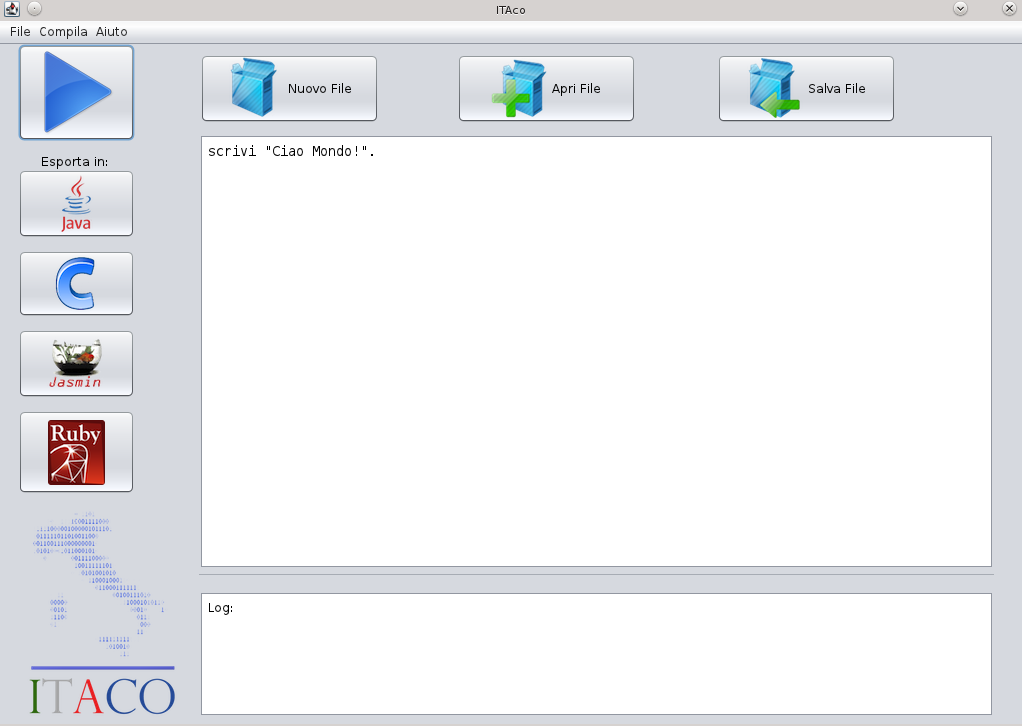
\includegraphics[scale=0.5]{img/gui_itaco.png}
\caption{Finestra principale della GUI}
\end{figure}

\subsection{Command Line Interface}
Oltre all'interfaccia grafica è stato ritenuto importante non tralasciare un
tool da riga di comando\footnote{in seguito ci si riferirà a tale strumento
con \emph{CLI}} che, sebbene possa essere meno intuitivo per il target di utenza
con poca dimestichezza all'utilizzo dei calcolatori, ridimensiona notevolmente
il problema di portabilità della \emph{GUI}, essendo la \emph{CLI} utilizzabile
in ogni sistema su cui sia presente l'ambiene Java.
\\Per avviare l'interfaccia a riga di comando è sufficiente avviare il file .jar
con almeno un parametro:
\begin{verbatim}
          java -jar itaco.jar nome_file_da_compilare.ita [linguaggio_target]
\end{verbatim}
il secondo parametro è opzionale. Nel caso della sua mancanza verrà generato
solo il codice .class.
\\La \emph{CLI} quindi aggiunge maggiore portabilità e la
possibilità di essere inserita in script.

\end{document}
